
\documentclass[withoutpreface,bwprint]{cumcmthesis} %去掉封面与编号页
\usepackage[final]{pdfpages}
\title{《软件需求工程 B》 大作业课题}
\tihao{A}
\baominghao{4321}
\schoolname{武汉理工大学}
\membera{小米}
\memberb{向左}
\memberc{哈哈}
\supervisor{老师}
\yearinput{2017}
\monthinput{08}
\dayinput{22}

\begin{document}

% \maketitle
%  \begin{abstract}
% 随着大数据时代数据量的不断膨胀,如何筛选及获取有效信息成为了一项重要技
% 能。 

% \keywords{\TeX{}\quad  图片\quad   表格\quad  公式}
% \end{abstract}

\includepdf{CoverOfBigHomework.pdf} 
\newpage
%目录
\tableofcontents

\newpage

\section{《人人都是产品经理》读书报告}

《人人都是产品经理》是苏杰的第一本书。该书从产品经理的岗位职责和自我
修养,需求的挖掘,项目的推进,团队的协作等方面展开,把产品经理的前世
今生剥开来,咽下去。
\begin{figure}[H]
	\centering
	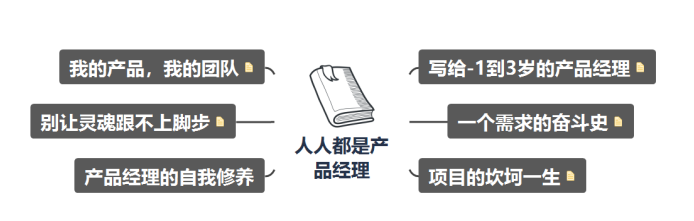
\includegraphics[width=12cm]{Snipaste_2019-09-19_19-31-46.png}
	\caption{ 《人人都是产品经理》思维导图 \label{fig:1}}
\end{figure}

产品经理指的是能够发新问题并描述清楚,转化为一个需求,进而转化为一个任务,争取到支持,发动一批人,并持续不断以主人翁的心态去跟踪,维护这个产物。

在我看来,相对于传统行业,互联网行业对于产品经理的要求与日俱增。在产品的设计过程中,用户对产品的习惯并没有产生较大的
依赖性,要求产品经理先入为主,主导用户习惯。在产品的研发过程中,需求设计分析的细节也显得尤为重要。此外,由于
互联网软件行业的生命周期较短,产品的更新迭代时长往往只有几个周甚至几天,所以要在项目完成度和产品质量之间找到平衡。

产品从广义上可以理解为解决某个问题的东西,而产品经理则是提供创意并打磨好这个东西的人。
书中从需求获取,分析,转化,测试等几个环节展示了产品经理眼中的需求。
也让我认识到产品经理需要具备很强的需求分析的能力,例如:
\begin{itemize}
\item \textbf{需求采集能力:} 需要把用户需求转化为产品需求,需要确定需求的基本属性,分析需求的商业价值,初评需求的实现难度,计算出它的性价比,并作出合理取舍。
\item \textbf{数据分析能力:}需要在对产品足够熟悉的基础上,先做出方向性的假设,再提取相应的数据并分析,得到一些现象, 最好是之前没发现的现象,然后尝试解释,接下来做用户调研修正解释,最终得出产品的最终发展方向。
\end{itemize}

做产品与做项目有很多不同点:从生命周期的角度来看,产品的生命周期相对更长,关注的市场品的整
个过程;产品需要不断地随着内外部变化进行修正;
从产出物的角度来看,产品是可批量生产,相对通用的。

因此产品经理与项目经理的要求也不尽相同,而让产品经理管理项目的目的,是希望能够在商业目标、项目资源、用户体验等各种限制条
件下取得平衡,解决目标不一致的问题,最重要的是必须在产品功能特征满足用户需求的前提下以及项目如
期完成的冲突中取得平衡。

\section{软件需求工程课程思考}
\subsection{需求优先级排序问题}

优先级难以进行抉择可能有以下\textbf{原因}:
\begin{itemize}
\item 需求分析人员对项目整体目标不明确,不能分清重要部分和紧急部分。
\item 需求列表有部分冗余信息,干扰了需求分析人员的判断。因此需要重新整理需求列表,化繁去简。
\item 需求分析系人员对需求掌握不深,没有挖掘各个需求的内在价值,对项目产生的影响,完成需求的风险。

\end{itemize}

现阶段下,这类需求优先级问题可以有由很多方法解决,例如:
层次分析法,产成本价值法,二叉树排序法,投票制度,一百元测试法,广数值分配法等。上述方法比较结果可得出:

\begin{table}[!htbp]
    \caption{各优先级技术比较}\label{tab:001} \centering
    \begin{tabular}{ccccc}
        \toprule[1.5pt]
        技术 & 度量 & 测量水平 & 复杂度 & 决策因素 \\
        \midrule[1pt]
        层次分析 & 定比尺度 & 细 & 非常复杂 & 战略重要性、损失\\
        累积投票 & 定比尺度 & 细 & 复杂 & 客户重要性\\
        二叉树 & 定序尺度 & 细 & 复杂 &  易变\\
        数值分配 & 定序尺度 & 粗 & 非常容易 & 时间、风险 \\
        \bottomrule[1.5pt]
    \end{tabular}
\end{table}

因此现阶段\textbf{层次分析法}更广泛用于\textbf{需求优先级决策},可以
首先根据需求建立递阶层次结构模型, 模型包含如下三个层次:
\begin{itemize}
\item 目标层.只有一个元素, 分析问题的预定目标或理想结果。

\item 准则层.包括为实现目标所涉及的中间环节, 它可由若干层次组成, 包括所需考虑
的准则、子准则,一般地, 软件需求优先级评定主要有三个指标:价值 v、费用 c 、风险 r。

\item 方案层.表示为实现目标可供选择的各种措施、决策方案等.这里是指需求分析中得到的各种需求.
\end{itemize}

并构造两两比较判断矩阵并计算单一准则下各个需求的相对权重,根据计算一致性检验
的比例来得到需求优先级排序。

\subsection{需求分析员必备的知识和技能}

\subsubsection{需求分析员岗位要求}
\begin{enumerate}
\item 独立完成用户需求的收集、整理、沟通、确认、分析等工作;
\item 根据用户需求,独立完成产品的原型、流程和交互界面设计,编写完整的产品需求规格说明书工作;
\item 独立完成已上线产品的功能优化和用户体验改进工作;
\item 独立完成项目需求文档及解决方案等相关文件的书写编制工作;
\item 较强的系统分析能力及文档编写能力;
\item 精通Axure、Mindmanager、PPT、Excel、Word等相关工具;
\end{enumerate}

\subsubsection{如何做好需求分析员}
从各大招聘网站上获得未来职业发展必备的知识和技能是较为直接的途径。
因此,在我看来需求分析员必备的知识或技能有:
\begin{itemize}
    \item 倾听、交谈和提问的技巧,分析、协调、观察、写作、组织、建模、人际交往能力和创造能力等。
    \item 具备各项实践经验中积累的广博知识,掌握相关领域的应用知识。
    \item 善于寻找处理问题的捷径,找到问题的本质。
    \item 分清问题的优先级,能够在恰当的时间处理好恰当的事情。
    \item 理解社会学、心理学,能够把握用户内心的需求,抓住用户动机。
\end{itemize}
\begin{figure}[H]
	\centering
	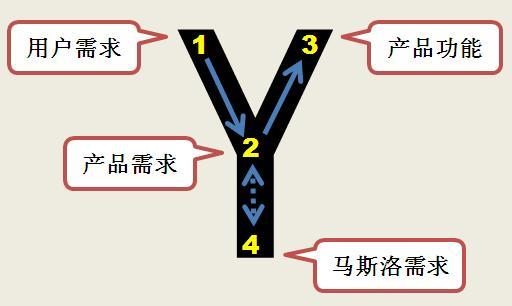
\includegraphics[width=12cm]{xuqiu.jpg}
	\caption{ 需求分析过程 \label{fig:1}}
\end{figure}

如图 2 是苏杰在《人人都是产品经理》上描述的需求的四个阶段,要做好需求分析员不是一蹴而就的事情,
需要我们在实践中逐步摸索,精益求精。
\section{案例分析}

\subsection{案例一}

首先我认为校园帮取快递的业务格局较小,在自动化物流飞速发展的今天,由人取快递极易被智能派送的方式取代。
因此我认为仅依靠校园送货上门服务
为载体的产品存在较大的局限性,必须与其他O2O服务(购物,餐饮,打印,校园服务)相结合才能有更好的发展。
\subsubsection{竞品分析}

\textbf{1.智能快递柜、智能"快递员"}

作为新一代智能物流体系,现阶段涌现了众多快递智能解决方案,其中包括:联邦快递、Amazon和京东的
智能"快递员"、菜鸟包裹和丰巢的智能快递柜(寄件人投递快递件到快递收发机;
快递服务人员收取快递件并运送至物流中心;物流中心通过快递服务人员派送快递件到相应的快递收发机;
收件人在附近的智能快递柜领取快递件)。
\begin{figure}[!h]
    \centering
    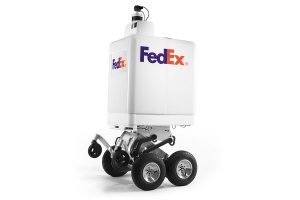
\includegraphics[width=.6\textwidth]{FedExBot.jpg}
    \caption{联邦快递—自动派送机器人}
    \label{fig:circuit-diagram}
\end{figure}

顶级物流服务主要体现在投入大,智能化程度高,终端大数据平台加持的特点。
因此在市场上的冲击下,校园帮取快递服务可替代性较强,缺乏核心竞争力。

\textbf{2.饿了么}

物流业务发展至今,餐饮外卖行业市场可能已经走向成熟,餐饮外卖业务也已成为校园O2O生活服务类别下重要的消费场景。
以武汉为例,单就校园快递/外卖而言,便捷的配送服务覆盖了各种餐饮,家具,生活用品,医疗药品等范围。
更有着庞大的配送物流体系以及较低的服务费用和较高的用户粘性。笔者曾使用饿了么下单购买药品,20分钟后在教学楼收到药品,配送费仅为0.1元;
也曾在夜间委托外卖小哥送夜宵,配送价格在2-8元不等。因此从身边案例来看,在物流较发达地区,配送服务并不具备议价能力,在没有技术壁垒、用户口碑的条件下很难占有市场。

\textbf{3.同类产品}
\begin{table}[!htbp]
    \caption{同类产品比较}\label{tab:001} \centering
    \begin{tabular}{ccccc}
        \toprule[1.5pt]
        功能 & 斑马校园 & 校园食堂外卖  \\
        \midrule[1pt]
        校园快递 & √ & √ \\
        校园商城 & √ & √ \\
        云打印 &  & √ \\
        互动课堂 &  & √  \\
        代取快递 &  √  & √ \\ 
        二手市场 &    &    \\
        表白墙 &    &  √  \\
        生活缴费 &    &  √  \\
        校园兼职 &  √  & √   \\
        社区分享 & √  &  \\
        \bottomrule[1.5pt]
    \end{tabular}
\end{table}

从横向同类产品分析来看,产品大多数功能都可以由QQ、支付宝、美团、饿了么、闲鱼等APP代替,因此如何针对校园
特点提供个性化服务是提高产品的市场占有率的重点问题。
\subsubsection{功能分析}
新软件的功能应包含以下几点:
\begin{itemize}
    \item 在校生学习服务,例如:查看课程表,查询成绩,查询考试安排等。
    \item 学校周边生活服务,例如:二手市场,帮取快递,社区分享,云打印等。
    \item 金融服务,例如:贷款,兼职平台,房屋租赁等。
    \end{itemize}
    \newpage
\subsubsection{产品亮点}
综上所述,我认为校园帮取快递APP缺乏市场活力,不益作为单例讨论。
校园产品亮点可以从两方面进行考虑:
\begin{itemize}
    \item 为在校生提供学习,生活等一站式服务平台,抓住校园特点,因地制宜提供特色服务。
    \item 为在校生提供安全可靠的金融、兼职服务平台。在花呗等借贷浪潮下让校园贷变得规范化,为大学生提供
    必要的安全后备金。
    \end{itemize}


\subsection{案例二}
化验单查读APP在市面上已有较为成熟的应用,例如:拍医拍、看懂化验单、云医拍等应用,可以看到,医疗+人工智能刚刚走上风口,
已有大量ToC,ToB的智能医疗解决方案涌现出来。
\begin{figure}[H]
	\centering
    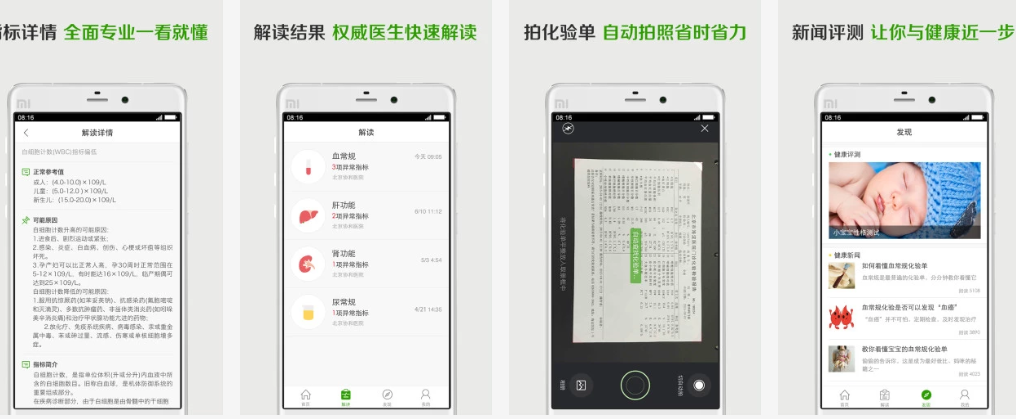
\includegraphics[width=16cm]{paiyipai.png}
	\caption{ 拍医拍解决方案 \label{fig:1}}
\end{figure}

\begin{itemize}
\item \textbf{背景问题} 实际上是患者和化验单的专业知识之间信息的不对称问题。
\item \textbf{业务目标:}从上传化验单到获得解读时间小于10分钟;APP上线第一周日活量2W+。
\item \textbf{用户群体:} 需要解读化验单的用户,包括糖尿病、心血管病等在内的慢病人群,软件为其长期提供化验单解读服务。
\item  \textbf{用户需求:} 解读化验单消耗时间少于10分钟;能够获得化验单各项指标的权威解读(包括:指标解释说明、列举大概会导致异常的原因和需要注意的事项);
                          能够整合往期化验单指标数据,可视化分析指标变化情况。
\item  \textbf{软件功能:} 拍照上传化验单;给出化验单各指标名词性解释、正常值范围;给出化验单综合解读结果并给出意见;提供权威医生线上解读服务
                          根据化验单历史数据进行比对分析,给出指导性意见。
\item  \textbf{非功能需求:} 用户在网络速度小于1Mb/s的条件下能够正常使用APP功能;化验单上传时具有加密功能;
                            各年龄段用户经过十分钟以内的学习后可以熟练使用APP。
\item  \textbf{原型界面:}   原型使用墨刀简易二次开发,项目详见(https://org.modao.cc/app/a41fbd2c58

dad5200d1dfca5689d1fd+5486ffbeb)
 
   \end{itemize}
   
\begin{figure}[H]
    \centering
    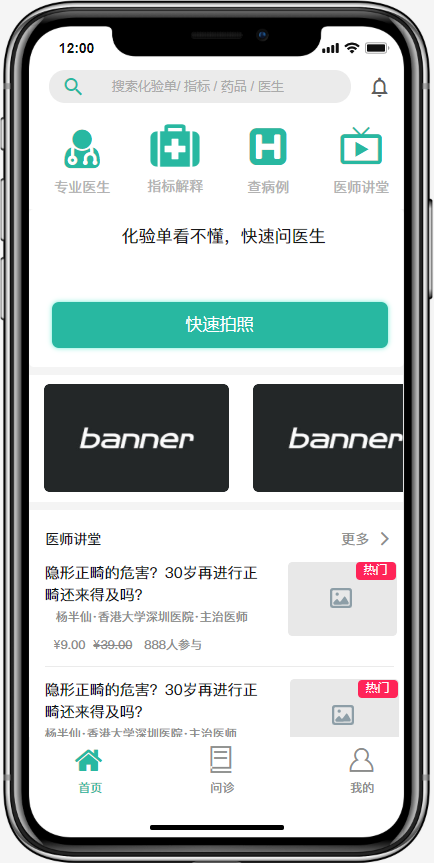
\includegraphics[width=.4\textwidth]{NP1.png}
    \caption{主页图}
    \label{fig:circuit-diagram}
\end{figure}

\begin{figure}[H]
    \centering
    \begin{minipage}[c]{0.4\textwidth}
        \centering
        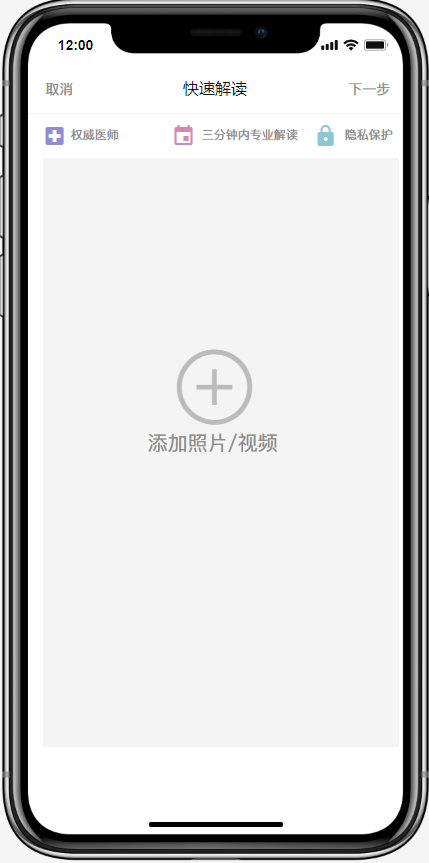
\includegraphics[height=0.5\textheight]{NP2.png}
        \subcaption{化验单拍照}
    \end{minipage}
    \begin{minipage}[c]{0.4\textwidth}
        \centering
        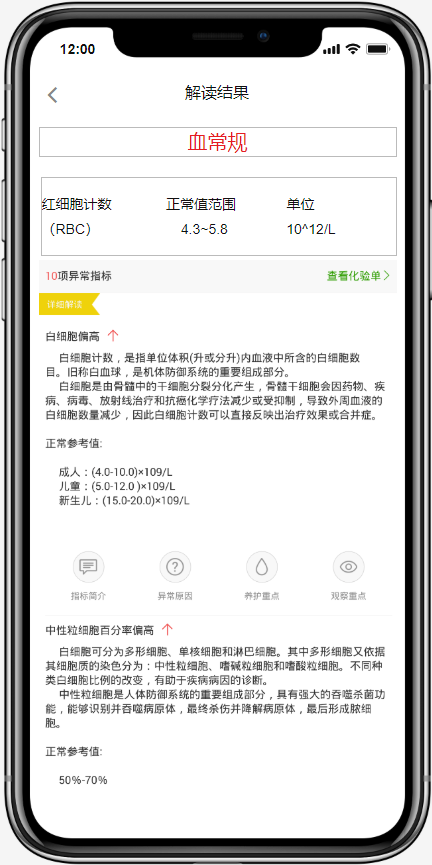
\includegraphics[height=0.5\textheight]{NP3.png}
        \subcaption{化验单解读}
    \end{minipage}
    \caption{主业务原型图}
\end{figure}

当用户拍照上传化验单后,APP会基于识别结果和历史学习经验进行预处理,并提交给医生进行逐条审核和再次加工,最终给出权威的解读报告,包括异常原因、养护重点、观察重点、指标简介、正常参考值等,并且每个化验单的报告都会持久地下来,并进行自动归类,方便用户随时查看。
    

\section{文献阅读报告}
眼动行为分析对于阅读行为,情感分析等各方面都有着重要的作用
,因此我阅读了一篇2018年基于眼动行为特征分析的事件检测算法的论文:Using machine learning to detect events in eye-tracking data (https://link.springer.com/article/10.3758/s13428-017-0860-3)
该篇论文发表于期刊Behavior Research Methods(ISSN: 1554-3528)。

其中,论文代码详见(https://github.com/r-zemblys/irf)。
数据集为Zemblys整理的眼动数据详见( https://doi.org/10.5281/zenodo.1343920 )

当前眼动追踪研究中的事件检测算法需要根据眼动数据调整
参数,本篇论文以人工标注的眼动事件数据为基础,训练了
IBF眼动事件的\textbf{通用分类器},在无需设置模型参数的情况下对注视
(fixations),扫视(saccades),扫视震荡(post-sacca
dic oscillations)等进行分类,并提供了
一个在眼动驱动的生物识别应用程序中采用该方法的示例。

论文主要分为以下三个步骤:
\begin{enumerate}
\item 提取插值之后的眼动行为数据特征,比如通过计算Input中的每个样本的凝视速度来计算速度特征,最终为每个样本生成14维特征向量

\item 以200棵决策树为初始训练阶段,并针对训练样本的随机子集(随机采样)进行完全分裂构建集合中的每个决策树,在机器学习中称为融合模型的装袋,最终构建完整的随机森铃分类模型。

\item 对分类器进行剪枝处理来减少模型的时间空间复杂度。最终得到了基于十个分类特征,十六棵决策树树建的随机森林分类模型。
\end{enumerate}

论文中还提到了进一步对其他眼动行为事件:视线平滑追踪(smooth pursuit)、眼球振颤(nystagmus),构建更完备的眼动行为事件分类模型。
     

\begin{figure}[H]
    \centering
    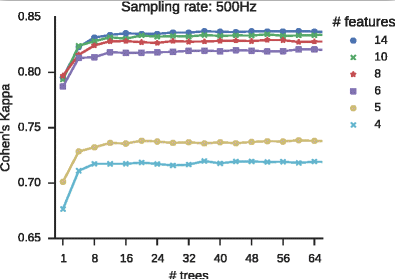
\includegraphics[width=0.8\textwidth]{ibfcut.png}
    \caption{分类器性能随特征数、决策树数变化图}
\end{figure}
这篇论文对眼动模型分类做了很详尽的阐述。
在保证模型性能的条件下减少模型的时间空间复杂度的分析过程也给了我很大的启发,如何在模型易推广,性能佳,可重用性强这几个目标下进行优化,也是机器学习中不可或缺的一部分。

\end{document}
